\documentclass{beamer}

% Input Encoding
\usepackage[utf8]{inputenc}

% PDF Bookmarks
\usepackage{url}
\usepackage{hyperref} 
\hypersetup{colorlinks}
\hypersetup{bookmarksopen}
\hypersetup{bookmarksnumbered}
\hypersetup{citecolor=blue}
\hypersetup{urlcolor=blue}
\hypersetup{linkcolor=blue}

% Spacing
\usepackage{xspace}

% Figures
\usepackage{graphicx}
\graphicspath{{img/}}
\usepackage{subcaption}

% Tables
\usepackage{booktabs}

% Strike Through
\usepackage{ulem}

% Code Snippet 
\usepackage{listings}
\lstset{
  belowcaptionskip=1\baselineskip,
  breaklines=true,
  frame=L,
  xleftmargin=\parindent,
  numbers=left,
  stepnumber=2,
  language=C,
  tabsize=2,
  showstringspaces=false,
  basicstyle=\footnotesize\ttfamily,
  keywordstyle=\bfseries\color{blue},
  commentstyle=\itshape\color{gray},
  identifierstyle=\bfseries\color{black},
  stringstyle=\bfseries\color{purple},
}

% Title
\title[Nanvix]{\textbf{The Nanvix Operating System}}

% Authors
\author[Pedro H. Penna]{%
	Pedro H. Penna%
}

% Affiliations
\institute{
	BSc. Computer Science\\
	\url{pedrohenriquepenna@gmail.com}
}

% Event.
\date[October 2016]{October 2016}

% Short-Hands
\newcommand{\ie}{\textit{ie.\xspace}}

% Agenda.
\AtBeginSection[]
{
	\begin{frame}
	\frametitle{Agenda}
		\tableofcontents[currentsection]
	\end{frame}
}

\begin{document}

\frame{\titlepage}

\section{Introduction}

		\begin{frame}
		\frametitle{Introduction}
		\framesubtitle{Context}
			\begin{itemize}
			\setlength\itemsep{1.5em}
				\uncover<1->{
					\item Early days of the Computer Era
					\begin{itemize}
					\setlength\itemsep{0.5em}
						\item Computers filled up entire rooms to perform
						simple calculations
						\item Programs were written in machine code
						\item Computer scientists had to deal with the bare
						hardware
					\end{itemize}
				}
				\uncover<2->{
					\item Information Era
					\begin{itemize}
					\setlength\itemsep{0.5em}
						\item Parallel architectures
						\item Large-scale distributed systems
						\item Modern programming languages
					\end{itemize}
				}
				\uncover<3->{
					\item What has enabled such evolution?
					\begin{itemize}
					\setlength\itemsep{0.5em}
						\item Computer abstractions
						\item Software stack
						hardware
					\end{itemize}
				}
			\end{itemize}
		\end{frame}

		\begin{frame}
		\frametitle{Introduction}
		\framesubtitle{Motivation}
			\begin{itemize}
			\setlength\itemsep{1.5em}
				\uncover<1->{
					\item Roles of an operating system
					\begin{itemize}
					\setlength\itemsep{0.5em}
						\item Multiplex access to resources
						\item Extend the functionalities of the underlying
					\end{itemize}
				}
				\uncover<2->{
					\item Expertise in operating systems
					\begin{itemize}
					\setlength\itemsep{0.5em}
						\item Design complex systems
						\item Master powerful mechanisms and strategies
						\item Deliver extra expertise in emerging topics
					\end{itemize}
				}
				\uncover<3->{
					\item Problems when learning about operating systems design
					\begin{itemize}
					\setlength\itemsep{0.5em}
						\item Simplistic, unrealistic or complex operating
						systems
						\item Lack in documentation and teaching material
					\end{itemize}
				}
			\end{itemize}
		\end{frame}

	\begin{frame}
	\frametitle{Agenda}
		\tableofcontents
	\end{frame}

\section{The Nanvix Operating System}

		\begin{frame}
		\frametitle{The Nanvix Operating System}
		\framesubtitle{Project Overview}
			\begin{itemize}
			\setlength\itemsep{0.5em}
				\item Created from scratch for educational purposes
				
				\item Designed to be small, simple, modern and fully featured
				
				\item Publicly available under the GPL v3 license at:
					\\[1em]
					\begin{center}
						\url{www.github.com/ppenna/nanvix}
					\end{center}
			\end{itemize}

			\begin{figure}[t]
				\captionsetup[subfigure]{
					justification=centering,
					labelformat=empty}
				\centering
					\begin{subfigure}{0.2\linewidth}
						
\includegraphics[width=\linewidth]{pedro}
						\caption{\scriptsize{Pedro H. Penna\\UFSC}}
					\end{subfigure}
					\quad
					\quad
					\begin{subfigure}{0.2\linewidth}
						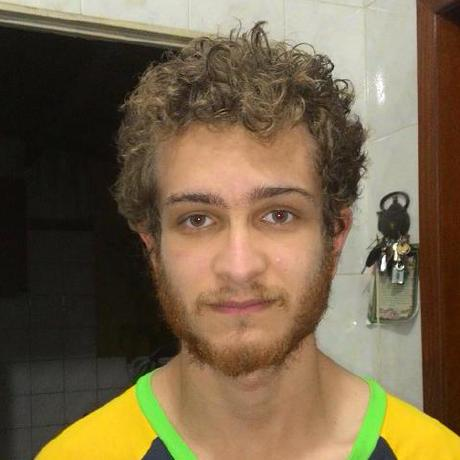
\includegraphics[width=\linewidth]{davidson}
						\caption{\scriptsize{Davidson Francis\\PUC Minas}}
					\end{subfigure}
					\quad
					\quad
					\begin{subfigure}{0.2\linewidth}
						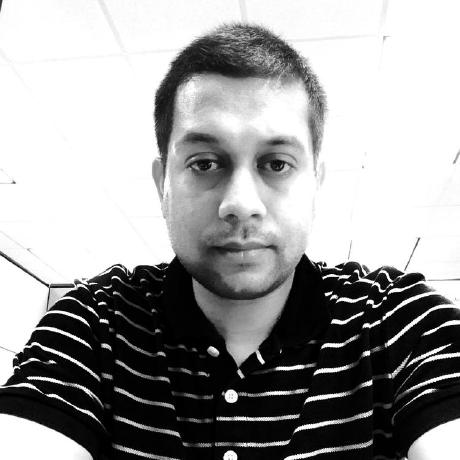
\includegraphics[width=\linewidth]{subhra}
						\caption{\scriptsize{Subhra Sarkar\\EchoStar Corp.}}
					\end{subfigure}
				\caption{People involved in the Nanvix Project.}
			\end{figure}
		\end{frame}

		\begin{frame}
		\frametitle{The Nanvix Operating System}
		\framesubtitle{Kernel Features}
			\begin{itemize}
			\setlength\itemsep{0.7em}
				\item POSIX compliant system call interface
				\item Unix System V architecture
				\item Non-preemptive
				\item Time-sharing
				\item Multiprogramming
				\item Interprocess communication
				\item Virtual memory with swapping
				\item Minix file system
				\item Uniform device interface
			\end{itemize}
		\end{frame}

		\begin{frame}
		\frametitle{The Nanvix Operating System}
		\framesubtitle{User-Land Features}
			\begin{itemize}
			\setlength\itemsep{0.5em}
				\item Standard C Library
				\item Unix-Like utilities

				\end{itemize}
				\begin{figure}
					\centering
					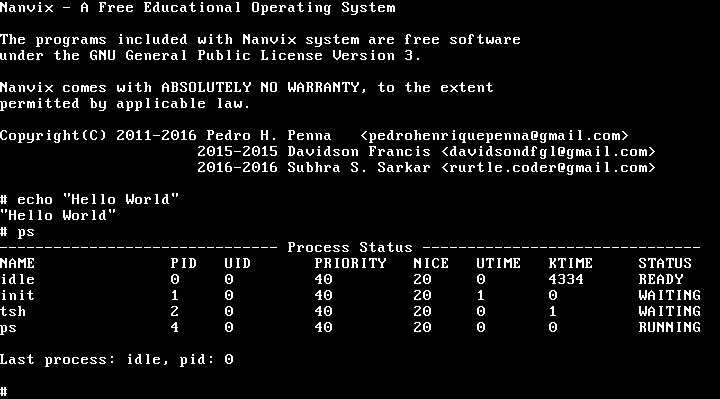
\includegraphics[width=0.8\textwidth]{nanvix}
					\caption{Nanvix running.}
				\end{figure}
		\end{frame}

\section{Baby Steps}

		\begin{frame}
		\frametitle{Baby Steps}
		\framesubtitle{Source Tree}
			\begin{itemize}
			\setlength\itemsep{0.6em}
			\footnotesize
				\uncover<1->{
					\item \texttt{bin}: binaries
				}
				\uncover<2->{
					\item \texttt{doc}: documentation
				}
				\uncover<3->{
					\item \texttt{include}
					\begin{itemize}
					\setlength\itemsep{0.2em}
					\footnotesize
						\item \texttt{include/dev}: device drivers headers
						\item \texttt{include/fs}: file systems headers
						\item \texttt{include/i386}: platform-specific headers
						\item \texttt{include/nanvix}: kernel headers
					\end{itemize}
				}
				\uncover<4->{
					\item \texttt{lib}: libraries
				}
				\uncover<5->{
					\item \texttt{src} 
					\begin{itemize}
					\setlength\itemsep{0.2em}
					\footnotesize
						\item \texttt{src/kernel}: kernel sources
						\item \texttt{src/lib}: libraries sources
						\item \texttt{src/sbin}: superuser utilities sources
						\item \texttt{src/ubin}: user utilities sources
					\end{itemize}
				}
			\end{itemize}
		\end{frame}

\begin{frame}[containsverbatim]
\frametitle{Baby Steps}
\framesubtitle{Building \& Running Nanvix}
	\begin{lstlisting}[language=bash,numbers=none,frame=single]
$ cd ~
$ git clone https://github.com/ppenna/nanvix
$ cd nanvix
$ sudo bash tools/dev/setup-toolchain.sh
$ sudo bash tools/dev/setup-bochs.sh
$ sudo reboot now
$ cd ~/nanvix
$ make nanvix
$ sudo make image
$ sudo bash tools/run/run.sh
	\end{lstlisting}
\end{frame}

\section{The Nanvix Kernel}

		\begin{frame}
		\frametitle{The Nanvix Kernel}
		\framesubtitle{Overview}
			\begin{figure}
				\centering
				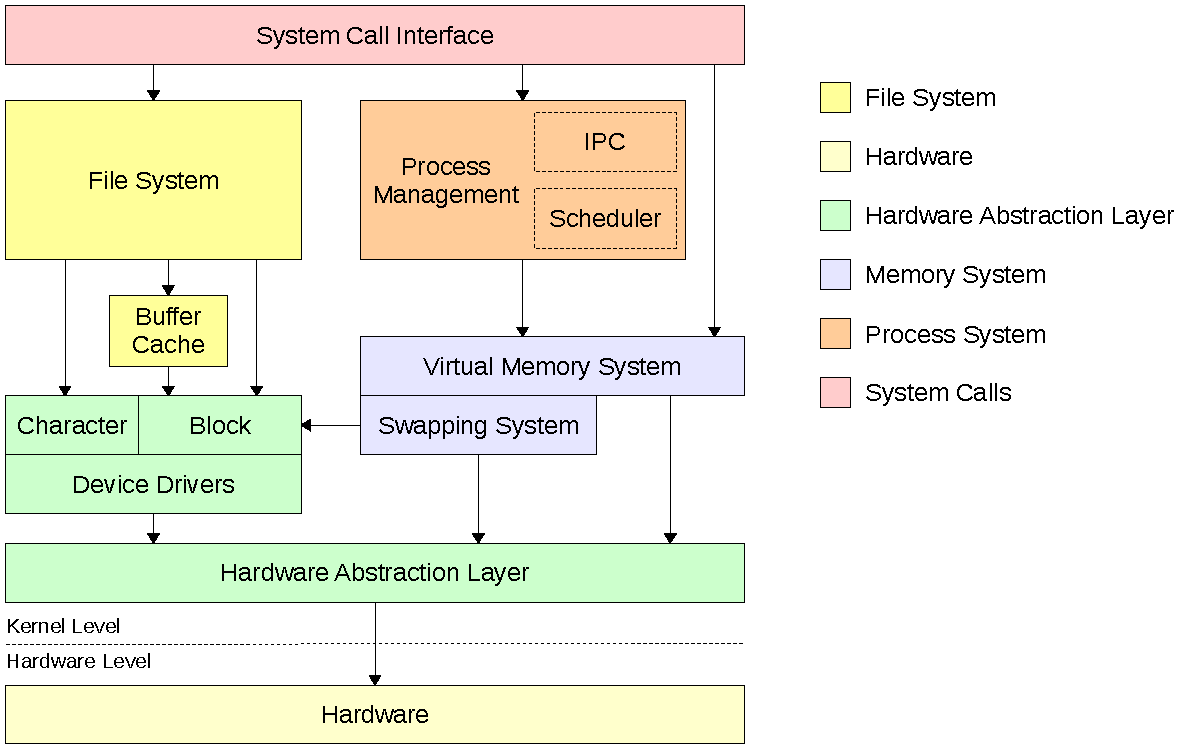
\includegraphics[width=\linewidth]{nanvix-architecture}
			\end{figure}
		\end{frame}

		\begin{frame}
		\frametitle{The Nanvix Kernel}
		\framesubtitle{Overview}
			\begin{table}
				\small
				\caption{Key system calls in Nanvix.}
				\begin{tabular}{l l l}
					\toprule
					\textbf{Category}  & \textbf{System Call(s)}   & \textbf{Description}             \\
					\midrule
					File System        & \texttt{open(), close()}  & Opens/Closes a File Descriptor   \\
					                   & \texttt{read(), write()}  & Reads/Writes to a File           \\
					                   & \texttt{link(), unlink()} & Creates/Removes a Link to a File \\ 
					                   & \texttt{stat()}           & Retrieves the Status of a File   \\
					                   & \texttt{chown()}          & Changes the File Ownership       \\[0.5em] 
					Process            & \texttt{fork()}           & Creates a Process                \\
					Management         & \texttt{execve()}         & Executes a Program               \\ 
					                   & \texttt{kill()}           & Sends a Signal to a Process      \\ 
					                   & \texttt{pause(), exit()}  & Suspends/Terminates the Process  \\ 
					\bottomrule
				\end{tabular}
			\end{table}
		\end{frame}

		\begin{frame}
		\frametitle{The Nanvix Kernel}
		\framesubtitle{The Process Management Subsystem}
			\begin{table}
				\caption{Key fields in a Process Control Block in Nanvix.}
				\begin{tabular}{l l l}
					\toprule
					\textbf{Category}  & \textbf{Field}   & \textbf{Description}      \\
					\midrule
					Context Switch     & \texttt{kstack}  & Kernel Stack              \\[0.4em]
					File System        & \texttt{pwd}     & Current Working Directory \\
					                   & \texttt{ofiles}  & Opened Files              \\[0.4em] 
					Memory Management  & \texttt{pregs}   & Memory Regions            \\ 
					                   & \texttt{pgdir}   & Page Directory            \\[0.4em]
					Process Management & \texttt{state}   & Current State             \\ 
					                   & \texttt{counter} & Remaining Quantum         \\ 
					                   & \texttt{pid}     & Process ID                \\ 
					                   & \texttt{nice}    & User-Level Priority       \\ 
					\bottomrule
				\end{tabular}
			\end{table}
		\end{frame}

		\begin{frame}
		\frametitle{The Nanvix Kernel}
		\framesubtitle{The Process Management Subsystem}
			\begin{figure}
				\centering
				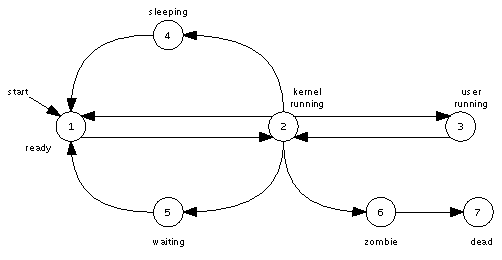
\includegraphics[width=\linewidth]{process-states}
				\caption{Figure: Life cycle of a process in Nanvix.}
			\end{figure}
		\end{frame}

		\begin{frame}[containsverbatim]
		\frametitle{The Nanvix Kernel}
		\framesubtitle{The Process Management Subsystem}
	\begin{lstlisting}[language=bash,numbers=none,frame=single]
PUBLIC void yield(void) {
	struct process *p, *next = IDLE;

	if (curr_proc->state == PROC_RUNNING)
		sched(curr_proc);

	for (p = FIRST_PROC; p <= LAST_PROC; p++) {
		if (p->state != PROC_READY)
			continue;
		if (p->counter > next->counter) {
			next->counter++; next = p;
			continue;
		}
			
		p->counter++;
	}
	
	switch_to(next);
}
	\end{lstlisting}
\end{frame}

		\begin{frame}
		\frametitle{The Nanvix Kernel}
		\framesubtitle{The Memory Management Subsystem}
			\begin{figure}
				\centering
				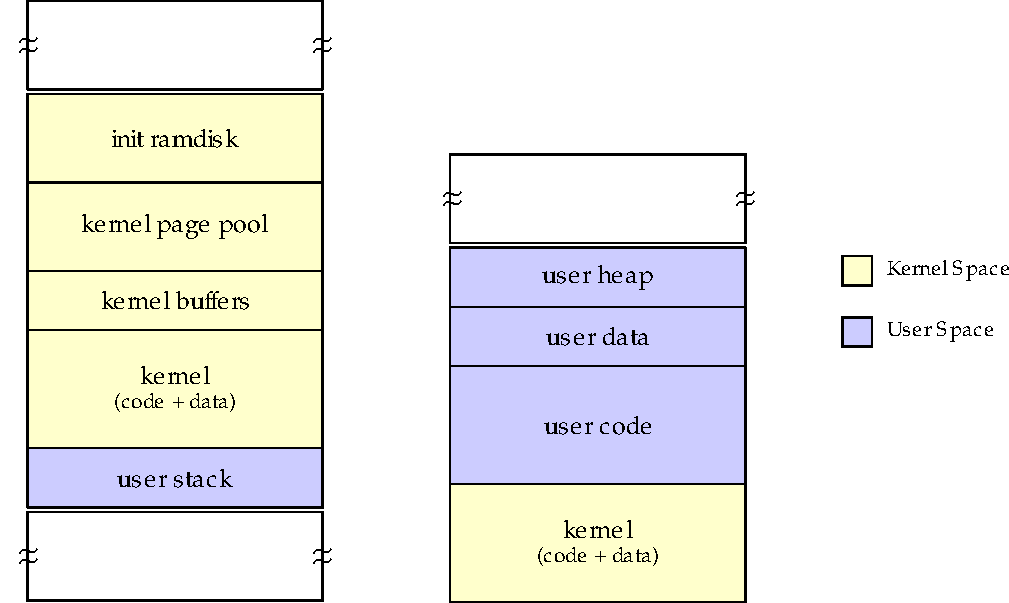
\includegraphics[width=0.9\linewidth]{memory-layout}
				\caption{Memory layout in Nanvix.}
			\end{figure}
		\end{frame}

		\begin{frame}
		\frametitle{The Nanvix Kernel}
		\framesubtitle{The Memory Management Subsystem}
			\begin{figure}
				\centering
				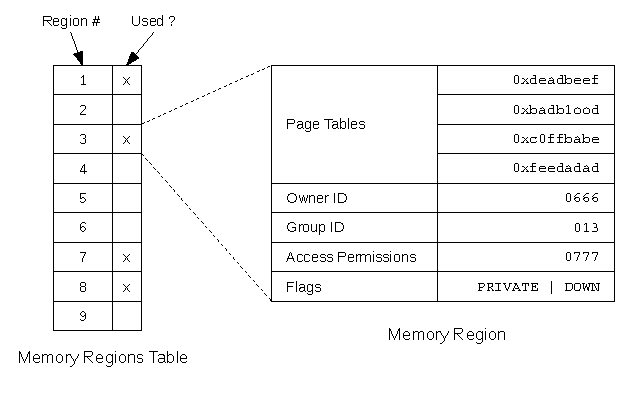
\includegraphics[width=\linewidth]{memory-regions}
				\caption{Memory regions in Nanvix.}
			\end{figure}
		\end{frame}

		\begin{frame}
		\frametitle{The Nanvix Kernel}
		\framesubtitle{The Memory Management Subsystem}
			\begin{figure}
				\centering
				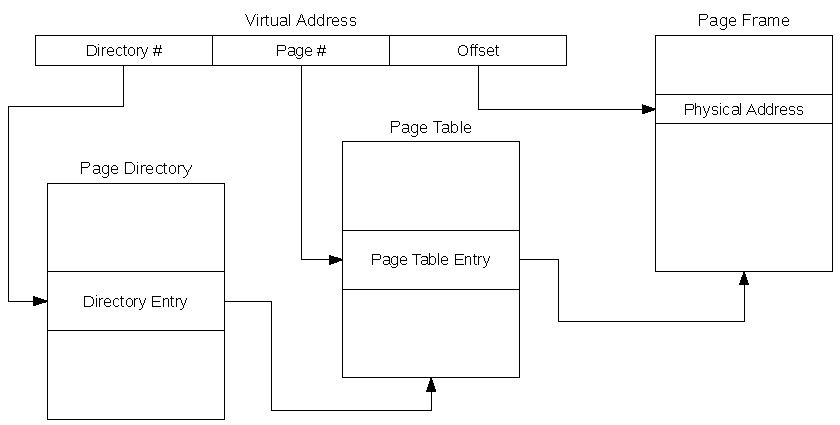
\includegraphics[width=\linewidth]{paging-scheme}
				\caption{Paging scheme used in Nanvix.}
			\end{figure}
		\end{frame}

		\begin{frame}
		\frametitle{The Nanvix Kernel}
		\framesubtitle{The Memory Management Subsystem}
			\begin{figure}
				\centering
				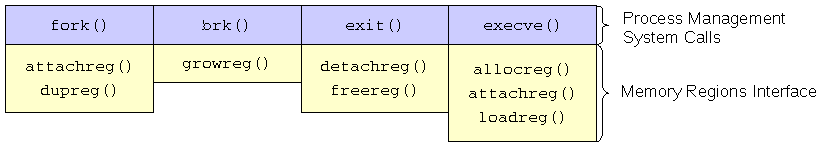
\includegraphics[width=\linewidth]{memory-regions-interface}
				\caption{Memory regions interface in Nanvix.}
			\end{figure}
		\end{frame}

		\begin{frame}
		\frametitle{The Nanvix Kernel}
		\framesubtitle{The File System}
			\begin{itemize}
			\setlength\itemsep{1.5em}
				\item Hierarchical file system
				\item Inodes hold metainformation about files
			\end{itemize}
			\begin{figure}
				\centering
				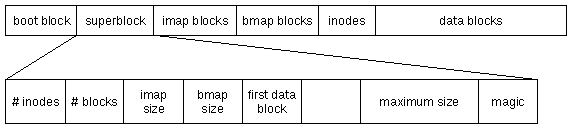
\includegraphics[width=\linewidth]{file-system-layout}
				\caption{Nanvix file system layout.}
			\end{figure}
		\end{frame}

		\begin{frame}
		\frametitle{The Nanvix Kernel}
		\framesubtitle{The File System}
			\begin{figure}
				\centering
				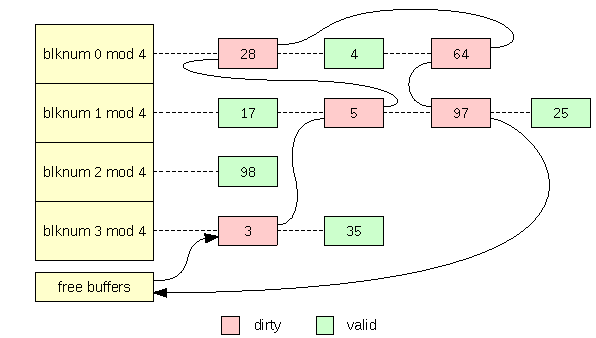
\includegraphics[width=\linewidth]{buffer-cache}
				\caption{The buffer cache subsystem.}
			\end{figure}
		\end{frame}

\section{Perspectives}

		\begin{frame}
		\frametitle{Perspectives}
		\framesubtitle{High Performance Computing}
			\begin{itemize}
			\setlength\itemsep{0.5em}
				\item \alert<1>{Manycore architectures}
				\item \alert<2>{Heterogeneous architectures}
				\item \alert<3>{Reconfigurable platforms}
			\end{itemize}
			\only<1>{
			\begin{figure}
				\centering
				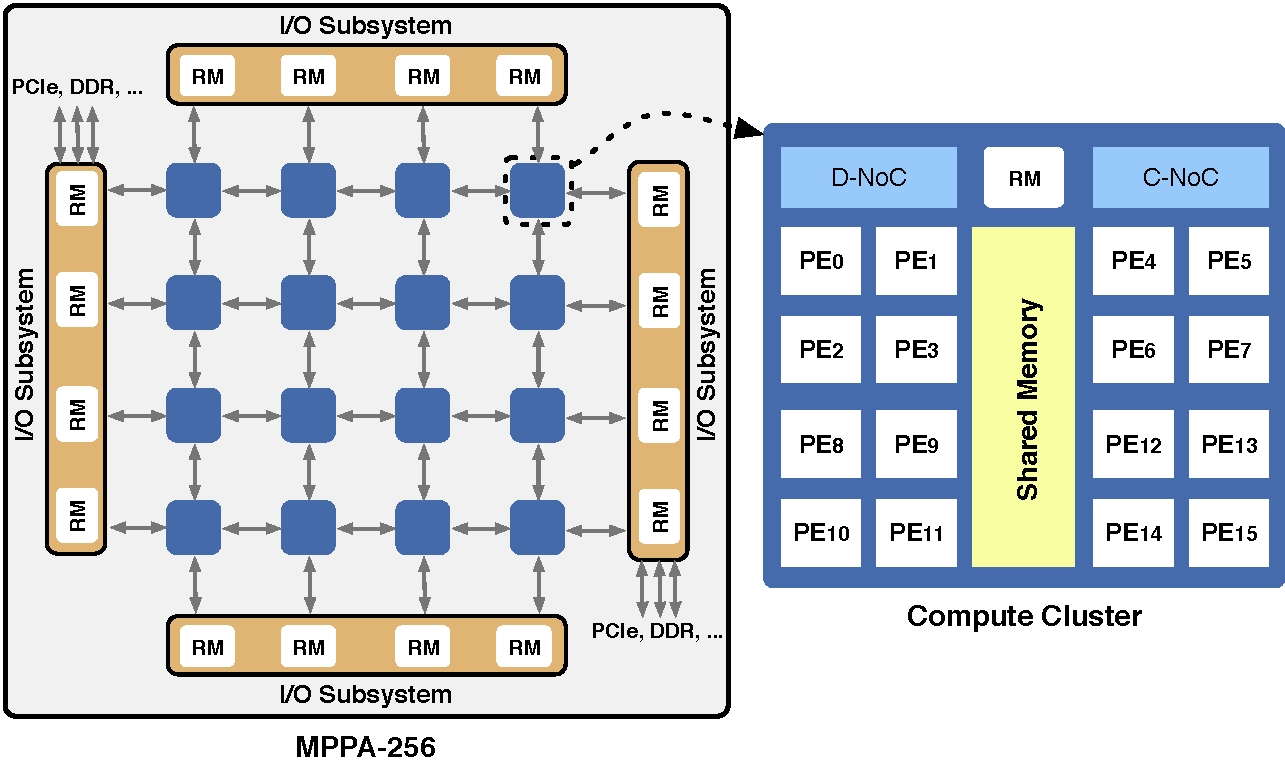
\includegraphics[width=0.6\linewidth]{mppa256}
				\caption{Kalray's MPPA-256 manycore processor}
			\end{figure}
			}
			\only<2>{
			\begin{figure}
				\centering
				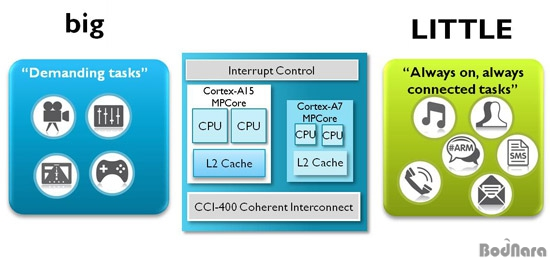
\includegraphics[width=0.6\linewidth]{big-little}
				\caption{Kalray's MPPA-256 manycore processor}
			\end{figure}
			}
			\only<3>{
			\begin{figure}
				\centering
				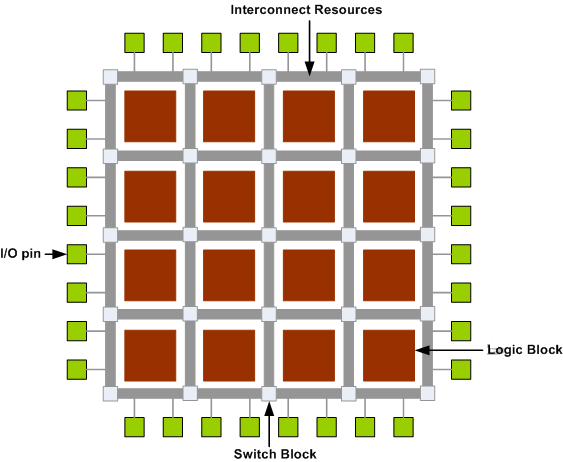
\includegraphics[width=0.45\linewidth]{fpga}
				\caption{Kalray's MPPA-256 manycore processor}
			\end{figure}
			}
		\end{frame}

		\begin{frame}
		\frametitle{Perspectives}
		\framesubtitle{Manycore Architectures}
			\begin{itemize}
			\setlength\itemsep{1.5em}
				\uncover<1->{
					\item \only<1>{Enhance the memory management subsystem}
					      \only<2->{\sout{Enhance the memory management subsystem}}
					\begin{itemize}
						\item \only<1>{Mini-regions}
						      \only<2->{\sout{Mini-regions}}
					\end{itemize}
				}
				\uncover<2->{
					\item \only<2>{Port user-level software}
					      \only<3->{Port user-level software (ongoing)}
					\begin{itemize}
						\item Newlib C Library
						\item Assembler, Compiler \& Linker
					\end{itemize}
				}
				\uncover<3->{
					\item Add multithreading support
					\begin{itemize}
					\setlength\itemsep{0.5em}
						\item Kernel threads
					\end{itemize}
				}
				\uncover<4->{
					\item Add message passing support
					\begin{itemize}
					\setlength\itemsep{0.5em}
						\item Light-weight MPI implementation
					\end{itemize}
				}
			\end{itemize}
		\end{frame}

\end{document}
